\documentclass[12pt, letter]{article}
\usepackage{graphicx} % Required for inserting images
\usepackage[letter, margin=1in]{geometry}
%\usepackage{paracol}
\usepackage{setspace}
\usepackage{graphicx}
\usepackage{wrapfig}
%\graphicspath{ {./images/} }
\usepackage{amsmath}
\usepackage{underscore}
\usepackage{hyperref}
\usepackage{listings}

\setlength\parindent{24pt}

\begin{doublespacing}
\title{Advancing Intelligence: Neural Networks
}
\author{Logan Endes \\ Department of Computer Science, RCBC \\ SRS 250 Intermediate Student Research \\ Professor Christopher Simber}
\date{May 3, 2024}

\end{doublespacing}

\begin{document}

\maketitle


\break


\begin{abstract}

Computer systems and solutions are becoming more intelligent every day. From identifying objects in a video stream to generating a report on a collection of data to making data-informed decisions in assistance of the average person, artificial intelligence (AI), more specifically machine learning (ML), is used to create machines capable of simulating processes to make decisions, “think,” and act accordingly given relevant data. At the core of these intelligent computers, neural networks are the most common solution to solve problems without an exact solution. This research will explore the development of neural networks in languages such as Python, the most commonly used language for AI development for its ease of use and popular frameworks like PyTorch, and C++, an efficient object-oriented programming (OOP) language used as a foundation in the popular PyTorch framework.


\end{abstract}





\section{Introduction} 


In recent years, the field of artificial intelligence has skyrocketed in growth rate and popularity thanks to viral tools such as ChatGPT, which stems from the breakthrough in language model architecture due to the creation of transformers in the paper, “Attention is All You Need,” (Vaswani et. al.). Before focusing on big breakthroughs and state of the art software, however, it is important to understand where it all comes from. Stemming from the initial and inefficient model of a “neuron,” the Perceptron, machine learning algorithms allow computers to make informed decisions through a guess and check process of learning.


In order to actually program these machine learning models, engineers need to choose a programming language. While you can theoretically program a neural network in any programming language, the two most popular languages for machine learning are Python and C++. Python is popular for its simplicity and frameworks like PyTorch and TensorFlow, both of which allow for extremely simple model development, and provide the tools necessary to use the parallel processing power of Graphical Processing Units (GPUs) that exponentially increase speed in training and inference of neural networks. C++ is widely used due to its efficiency in system-level operations, and it is the language of which the popular framework PyTorch is built on. 


This paper aims to explain what a neural network is, the fundamental parts that make a neural network, and explore the practical aspects of implementing neural networks comparatively with Python and C++. 

\section{Neural Networks: An Overview}

	Neural networks are inspired by the biological networks of neurons that make up the brains of humans and other animals, hence the name. Following this theme, neural networks are a collection of neurons connected to each other in layers; in more technical terms, they are a sequence of simple processing nodes that can follow complex behavior depending on the weights and biases built into them as well as many other factors like number of layers and which layers are connected. At inception, neural networks are basically applying random linear algebra to whatever is inputted, and over time, they learn through a training process consisting of a guess and check method in which they slightly change the math applied in each neuron and check against pre-labeled data. As training continues, and assuming the problem is realistic for the neural network to solve, it will become more and more accurate until it is reliable in predicting an output based on the given input, this is the intelligence aspect of artificial intelligence. 

\begin{singlespacing}\subsection{The Perceptron}\end{singlespacing} 


Invented in 1958 by Frank Rosenblatt, the perceptron is the simplest type of neural network made up of a single neuron. The function of a perceptron is to perform what is known as binary classification: given one input, determine whether it does or does not fit in the category (or you could say it places it into one of two categories), this function of binary classification means that the perceptron is a type of linear classifier. As with most processes in the realm of machine learning, the perceptron can be translated to a mathematical model:

\begin{equation}
y = f(w^Tx+b)
\end{equation}

\noindent where w represents the weight vector, x the input vector, b the bias, and f the activation function. This can similarly be described as a type of linear regression problem, but that was not necessarily its original intended function. Along with its mathematical model, a perceptron is only able to learn thanks to its learning rule:

\begin{equation}
w_n_e_w = w_o_l_d + l(t-y)x
\end{equation}
	
\noindent where l is the learning rate, t is the true label, and y is the predicted label. 

With the creation of the perceptron, more complex neural networks were eventually able to be built with this as its foundation to learn more complex features of data, though it was not until decades later that researchers discovered the complex applications of this perceptron. 

\subsection{Feedforward Neural Networks}

In 1965, the idea came about connecting multiple layers of perceptrons together to complete more complex tasks in the form of the first feedforward neural network (Ivakhnenko). However, it was not until much later that the first feedforward neural network was implemented with the help of gradient descent in what is known as a backpropagation algorithm. By connecting multiple linear perceptrons, feedforward neural networks are able to identify non-linear relationships, greatly expanding the utility of machine learning and officially becoming the first deep neural network. One very simple example of a problem that requires non-linearity is the boolean XOR operator; you need three perceptrons to solve this: !AND, OR and AND, in which the former two will take the same input, and both will connect to the final AND perceptron to determine the XOR operation. 


\subsection{Architecture}

Feedforward neural networks have a more complex architecture than a simple single-node perceptron: they must have an input layer, one or more hidden layers, and an output layer which each have a certain number of neurons and are connected via weights which are modified as they travel through each layer. Each neuron in this multi-layer perceptron is a perceptron itself, and thus with many perceptrons connected, more complex tasks are able to be solved. 


\subsection{Processing}

In addition to a more complex architecture, there are more important and complex processes inside of feedforward neural networks: the forward pass and backpropagation. In the forward pass, input data is passed through each layer of the network and modified by each neuron’s activation function until it is finally outputted as a prediction. In backpropagation, the network adjusts each neuron's weights to calculate a more accurate prediction by calculating the gradient of the error function with respect to each weight as part of the learning phase, a common technique for this is known as gradient descent. 


\subsection{Optimization}

Inside feedforward neural networks, the actual "learning" takes place during backpropagation, which is split into a loss function step and an optimizer step. The loss function compares the predicted result to the pre-labeled data used for training and calculates a loss based on the difference of the two. With this loss value, the gradient descent optimizer iteratively adjusts the network's weights in the opposite direction of the gradient of the loss. Although this works in many cases, the gradient descent algorithm was later expanded into stochastic gradient descent due to it tending to converge towards suboptimal gradients and it being slow. The limitations of speed and inaccuracy led to more efficient optimizers that take into account momentum and adaptive learning rates. In this process of optimization as part of training a neural network, the learning rate, sometimes denoted epsilon, and initial weights play crucial roles. Epsilon determines the step size used while updating weights in the optimization process. If it is too large, the model will overshoot optimal values and cause unstable training, whereas if it is too small, optimization will become slow and settle in a local minima, leading to suboptimal weights and biases in the final neural network. The initial weights are important because they can lead to inefficient learning by the neural network with slow convergence on an optimal solution or getting trapped in local minima and suboptimal solutions similar to learning rates that are too small. Generally, weights are initialized with random values, but in more advanced networks, there are strategies for weight initialization that the into account the architecture of the neural network. 


\subsection{Activation Functions}

Activation functions determine how a neuron’s weighted calculation is transformed into an output, one of the most popular being the sigmoid function, which can be represented as:
\begin{equation}
\sigma(x)= \frac{1}{1+e^-^x}
\end{equation}
	
This function is popular due to its introduction of nonlinearity into linear outputs as well as its output being between 0 and 1, making it very useful for converting weighted sums into probabilities for classification problems. Despite its popularity, it suffers from limitations such as being prone to the vanishing gradient problem, its non-zero centered output makes training more difficult and unstable, and it can be more time consuming due to its use of power operations. 


\subsection{Training and Testing}

The ability of a neural network to make accurate predictions depends on the data used in the training and testing of the neural network. Training involves the process of making predictions with random weights and biases, comparing them to predetermined labels for each input, and adjusting the weights and biases inside of the neural network depending on the difference between the predicted labels and true training labels. Testing, on the other hand, introduces new, unseen data to the network and tracks its progress/accuracy in making predictions on the given inputs. Unlike during training, the weights and biases of the network are not modified during testing, and instead it is only used to evaluate the model’s ability to make correct predictions. 

In order to optimally train a neural network, it is important to properly split your data into training, validation, and testing datasets. If your data is not properly split and you, for example, are training on one specific type of data and trying to test it on data too dissimilar to the training set, you are likely to “overfit” on your training data, in which you will only be able to properly make predictions on a very specific type of data instead of the optimal generalized data that you should be able to predict on. With this in mind, it is important to diversify your dataset so it better fits to more generalized data and can accurately predict the desired data. 


\section{Development}

With this understanding of neural networks, you are now able to apply a neural network to solve a problem like predicting the function:

\begin{equation}
f(x) = sin(x)
\end{equation}
	
 
\noindent In this example, we will be using Python and the popular library, NumPy, made for scientific computing with Python written in C to provide more efficient functionality than native Python code. This following example is based on the article, “Simple MLP Backpropagation Artificial Neural Network in C++ (Step by Step),” (Haghrah). \\

First, you must import necessary libraries and modules:


\begin{lstlisting}[language=Python]
import numpy as np
import math
import time 
import random as rand
import matplotlib.pyplot as plt
\end{lstlisting}

\noindent In addition to numpy, we will be using matplotlib in order to plot the results of our neural network’s predictions in comparison to fixed labels as well as the math, time, and random modules.\\

Next, we will be instantiating global parameters known as hyperparameters, these include values like epsilon, the number of training cycles to run, and unpopulated global variables for the weights and biases of our neural network. 

\begin{lstlisting}[language=Python]
TRAIN_SET_SIZE = 50
PI = math.pi
N = 5
epsilon = 0.05
epoch = 50000

c = np.ndarray(N)
W = np.ndarray(N)
V = np.ndarray(N)
global b 
b = float(0)
\end{lstlisting}

For this neural network, we will be utilizing the sigmoid activation function as well as a forward pass function which can be mathematically represented as:

\begin{equation}
h=sigmoid(c+Wx)
\end{equation}
\begin{equation}
f(x)=b+Vh
\end{equation}
	
 
\noindent This function, f(x) is able to estimate the function sin(x), we can now represent all of this in code:

\begin{lstlisting}[language=Python]
def sigmoid(x: float) -> float:
    return (1.0 / (1.0 + math.exp(-x)))

def f_theta(x: float) -> float:
    result = b
    for i in range(N):
        result += V[i] * sigmoid(c[i] + W[i] * x)
    return result
\end{lstlisting}

In order to actually utilize these functions we’ve made and manipulate the weights and biases of our neural network, we need to create a function to train it and manipulate the weights based on the difference between predicted labels and actual values. Without going deep into the math behind this, we can program it as follows:

\begin{lstlisting}[language=Python]
def train(x: float, y: float):
    for i in range(N):
        W[i] = W[i] - epsilon * 2 * (f_theta(x) - y) * V[i] * x * \
        (1 - sigmoid(c[i] + W[i] * x)) * sigmoid(c[i] + W[i] * x)
    
    for i in range(N):
        V[i] = V[i] - epsilon * 2 * (f_theta(x) - y) * \
        sigmoid(c[i] + W[i] * x)

    global b
    b = b - epsilon * 2 * (f_theta(x) - y)

    for i in range(N):
        c[i] = c[i] - epsilon * 2 * (f_theta(x) - y) * V[i] * \
        (1 - sigmoid(c[i] + W[i] * x)) * sigmoid(c[i] + W[i] * x)

\end{lstlisting}

Now that we have the ability to train the network, we need to put it all together by setting the weights randomly, creating a training dataset, iterating through the training loop, and testing it with a different testing dataset; this is shown in the following main function:

\begin{lstlisting}[language=Python]
def main():
    rand.seed(time.time())
    start = time.perf_counter()
    for i in range(N):
        W[i] = 2 * rand.random() / 2147483647 - 1
        V[i] = 2 * rand.random() / 2147483647 - 1
        c[i] = 2 * rand.random() / 2147483647 - 1

    trainSet = np.empty((TRAIN_SET_SIZE, 2))
    
    for i in range(TRAIN_SET_SIZE):
        trainSet[i] = np.array(((i * 2 * PI / TRAIN_SET_SIZE), \
        math.sin(i * 2 * PI / TRAIN_SET_SIZE)))

    for i in range(epoch):
        for j in range(TRAIN_SET_SIZE):
            train(trainSet[j][0], trainSet[j][1])
        print("Epoch: ", i)
    total = time.perf_counter() - start
    print("Training took: ", total, " seconds.")

    x = np.empty(1000) # input
    y1 = np.empty(1000) # true labels
    y2 = np.empty(1000) # preds

    for i in range(1000):
        x[i] =  i * 2 * PI / 1000
        y1[i] = math.sin(i * 2 * PI / 1000)
        y2[i] = f_theta(i * 2 * PI / 1000)
    
    plt.figure(figsize=(10, 7))
    plt.scatter(x, y1, c="b", s=4, label="True Data")
    plt.scatter(x, y2, c="g", s=4, label="Predictions")
    print(x, y1, y2)
    plt.show()

\end{lstlisting}

If you’d like to use this code yourself, you can find it at \href{https://github.com/Log45/SRS-250}{https://github.com/Log45/SRS-250}. This specific example is under the file \href{https://github.com/Log45/SRS-250/blob/main/np_example.py}{np\_example.py}, the associated C++ example can be found under the file \href{https://github.com/Log45/SRS-250/blob/main/cpp_example.cpp}{cpp\_example.cpp}.

\section{Observations}

After running through this example, we were able to get the following results (Green=Predictions, Blue=Truth):


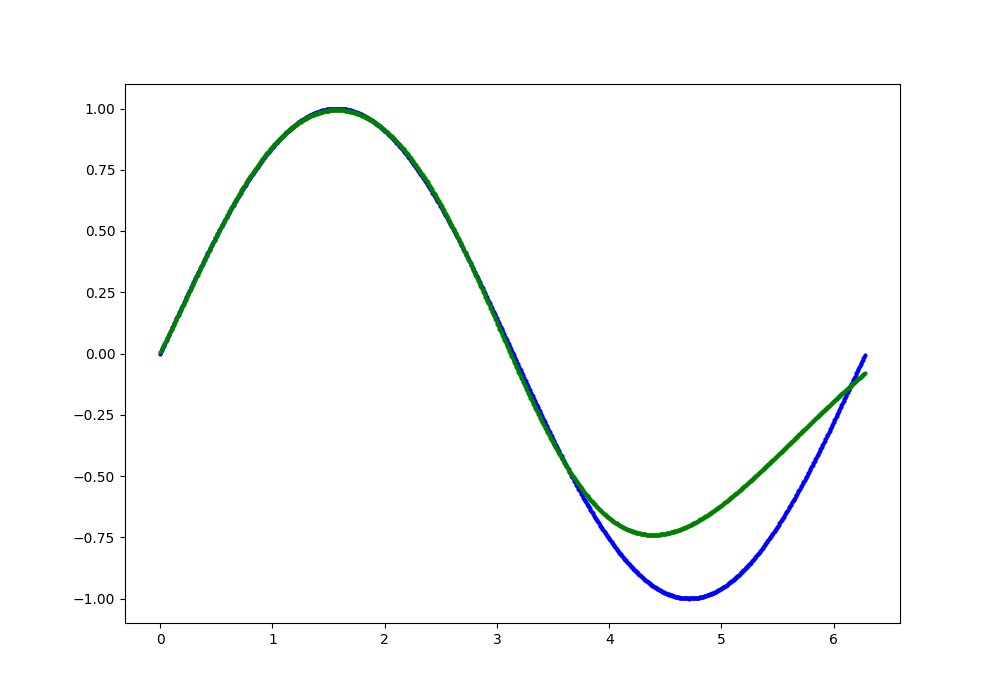
\includegraphics[width=.8\textwidth]{images/Figure_1.png}
\newline
\centering
\textbf{Epsilon=0.05} 

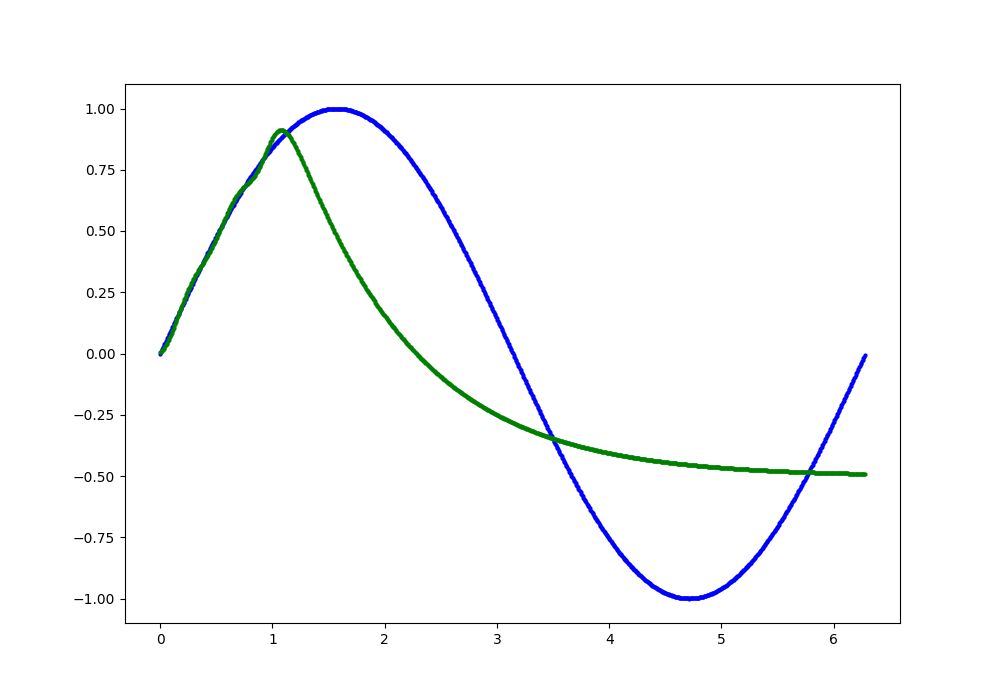
\includegraphics[width=.8\textwidth]{images/Figure_2.png}
\newline
\centering
\textbf{Epsilon=0.1} 

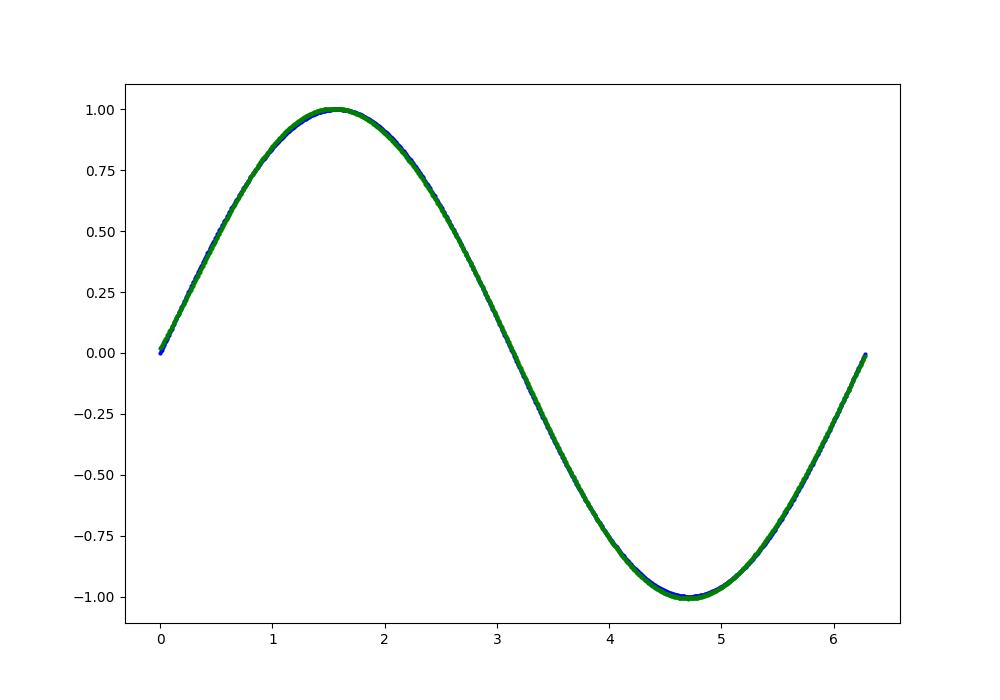
\includegraphics[width=.8\textwidth]{images/Figure_3.png}
\newline
\centering
\textbf{Epsilon=0.01} 

\break
\raggedright

\section{Summary}

In this paper, we explored the concepts of neural networks, the parts that make them, and a practical application of a neural network to predict the sin function. With the above implementation, we were able to reliably predict values of the sin function with near-exact accuracy. Along with this, we were also able to display the importance of the epsilon value in neural networks; as seen above, having too large of an epsilon value leads to very poor fitting and while a learning rate in the middle is decent, the smaller learning rate fits near-perfect to the true values of sin thanks to the large amount of training iterations. Compared to the C++ implementation based on the previously mentioned article (Haghrah) which can also be found in the github repository, the C++ implementation is slightly more efficient and for a reason that’s not entirely clear, was more accurate with the same parameters. Whereas the Python implementation consistently took about 120 seconds for the entire 50000 training epochs, the C++ implementation took a consistent 115 seconds on my computer. This slight difference can be attributed to the fact that the Python implementation used NumPy, which is implemented in C and thus much more efficient than native Python, but the fact that it is still a Python program makes it slightly less efficient than the pure C++ implementation. 
 
\newpage

\nocite{*}
\bibliographystyle{plain} % We choose the "plain" reference style
\bibliography{refs} % Entries are in the refs.bib file


\end{document}